\documentclass[14pt]{extbook}
\usepackage{multicol, enumerate, enumitem, hyperref, color, soul, setspace, parskip, fancyhdr} %General Packages
\usepackage{amssymb, amsthm, amsmath, latexsym, units, mathtools} %Math Packages
\everymath{\displaystyle} %All math in Display Style
% Packages with additional options
\usepackage[headsep=0.5cm,headheight=12pt, left=1 in,right= 1 in,top= 1 in,bottom= 1 in]{geometry}
\usepackage[usenames,dvipsnames]{xcolor}
\usepackage{dashrule}  % Package to use the command below to create lines between items
\newcommand{\litem}[1]{\item#1\hspace*{-1cm}\rule{\textwidth}{0.4pt}}
\pagestyle{fancy}
\lhead{Makeup Progress Quiz 2}
\chead{}
\rhead{Version C}
\lfoot{5763-3522}
\cfoot{}
\rfoot{Spring 2021}
\begin{document}

\begin{enumerate}
\litem{
Solve the equation below. Then, choose the interval that contains the solution.\[ -10(4x + 13) = -3(-19x -8) \]\begin{enumerate}[label=\Alph*.]
\item \( x \in [0.28, 1.11] \)
\item \( x \in [-1.38, -1.04] \)
\item \( x \in [6.02, 6.77] \)
\item \( x \in [-2.14, -1.5] \)
\item \( \text{There are no real solutions.} \)

\end{enumerate} }
\litem{
First, find the equation of the line containing the two points below. Then, write the equation as $ y=mx+b $ and choose the intervals that contain $m$ and $b$.\[ (-11, 10) \text{ and } (-6, 2) \]\begin{enumerate}[label=\Alph*.]
\item \( m \in [-1.1, 4.8] \hspace*{3mm} b \in [11.31, 11.94] \)
\item \( m \in [-2.3, 0.8] \hspace*{3mm} b \in [20.95, 21.07] \)
\item \( m \in [-2.3, 0.8] \hspace*{3mm} b \in [-7.92, -7.56] \)
\item \( m \in [-2.3, 0.8] \hspace*{3mm} b \in [7.98, 8.09] \)
\item \( m \in [-2.3, 0.8] \hspace*{3mm} b \in [7.4, 7.8] \)

\end{enumerate} }
\litem{
Find the equation of the line described below. Write the linear equation as $ y=mx+b $ and choose the intervals that contain $m$ and $b$.\[ \text{Parallel to } 9 x - 8 y = 12 \text{ and passing through the point } (-8, -5). \]\begin{enumerate}[label=\Alph*.]
\item \( m \in [0.91, 1.27] \hspace*{3mm} b \in [3.1, 5.4] \)
\item \( m \in [0.91, 1.27] \hspace*{3mm} b \in [-5.1, -2.9] \)
\item \( m \in [0.41, 0.98] \hspace*{3mm} b \in [3.1, 5.4] \)
\item \( m \in [0.91, 1.27] \hspace*{3mm} b \in [-0.3, 3.9] \)
\item \( m \in [-1.35, -0.78] \hspace*{3mm} b \in [-14.6, -13.7] \)

\end{enumerate} }
\litem{
Write the equation of the line in the graph below in Standard form $Ax+By=C$. Then, choose the intervals that contain $A, B, \text{ and } C$.
\begin{center}
    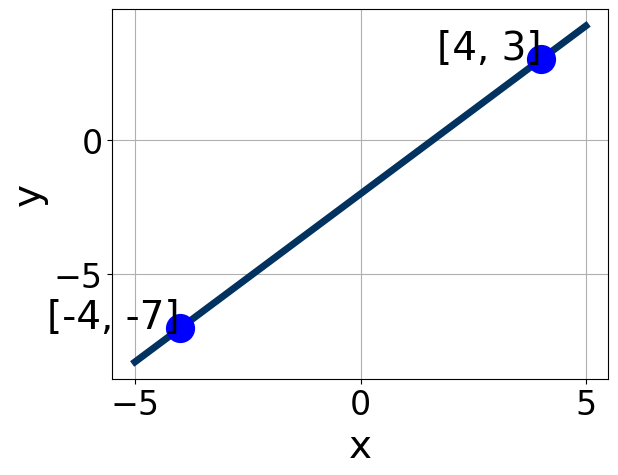
\includegraphics[width=0.5\textwidth]{../Figures/linearGraphToStandardCopyC.png}
\end{center}
\begin{enumerate}[label=\Alph*.]
\item \( A \in [2, 7], \hspace{3mm} B \in [-4.39, -2.68], \text{ and } \hspace{3mm} C \in [3, 14] \)
\item \( A \in [2, 7], \hspace{3mm} B \in [2.73, 4.14], \text{ and } \hspace{3mm} C \in [-10, -4] \)
\item \( A \in [-4.25, -0.25], \hspace{3mm} B \in [0.09, 1.09], \text{ and } \hspace{3mm} C \in [-7, 1] \)
\item \( A \in [-4.25, -0.25], \hspace{3mm} B \in [-1.42, -0.07], \text{ and } \hspace{3mm} C \in [1, 3] \)
\item \( A \in [-10, -3], \hspace{3mm} B \in [2.73, 4.14], \text{ and } \hspace{3mm} C \in [-10, -4] \)

\end{enumerate} }
\litem{
Write the equation of the line in the graph below in Standard form $Ax+By=C$. Then, choose the intervals that contain $A, B, \text{ and } C$.
\begin{center}
    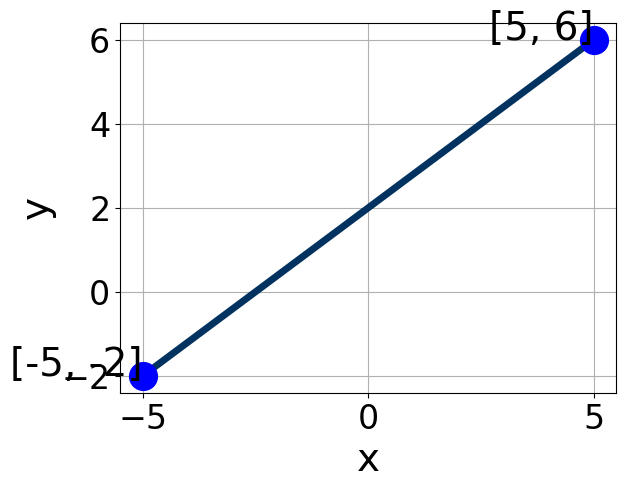
\includegraphics[width=0.5\textwidth]{../Figures/linearGraphToStandardC.png}
\end{center}
\begin{enumerate}[label=\Alph*.]
\item \( A \in [-0.8, 0.2], \hspace{3mm} B \in [-1.5, 0.1], \text{ and } \hspace{3mm} C \in [-2.2, -0.1] \)
\item \( A \in [4, 8], \hspace{3mm} B \in [2.9, 7.1], \text{ and } \hspace{3mm} C \in [9.6, 10.7] \)
\item \( A \in [-0.8, 0.2], \hspace{3mm} B \in [-0.5, 3], \text{ and } \hspace{3mm} C \in [-0.3, 2.7] \)
\item \( A \in [4, 8], \hspace{3mm} B \in [-6.7, -4.4], \text{ and } \hspace{3mm} C \in [-10.8, -8.7] \)
\item \( A \in [-10, -2], \hspace{3mm} B \in [2.9, 7.1], \text{ and } \hspace{3mm} C \in [9.6, 10.7] \)

\end{enumerate} }
\litem{
Solve the linear equation below. Then, choose the interval that contains the solution.\[ \frac{-4x + 9}{2} - \frac{3x + 3}{4} = \frac{-9x -5}{7} \]\begin{enumerate}[label=\Alph*.]
\item \( x \in [2.1, 3.8] \)
\item \( x \in [5.9, 7.7] \)
\item \( x \in [-3.1, -1.4] \)
\item \( x \in [3.5, 5.4] \)
\item \( \text{There are no real solutions.} \)

\end{enumerate} }
\litem{
Find the equation of the line described below. Write the linear equation as $ y=mx+b $ and choose the intervals that contain $m$ and $b$.\[ \text{Parallel to } 5 x + 9 y = 4 \text{ and passing through the point } (7, -10). \]\begin{enumerate}[label=\Alph*.]
\item \( m \in [-1.4, 0.3] \hspace*{3mm} b \in [-19, -16] \)
\item \( m \in [-4, -0.7] \hspace*{3mm} b \in [-7.11, 1.89] \)
\item \( m \in [-1.4, 0.3] \hspace*{3mm} b \in [4.11, 8.11] \)
\item \( m \in [-0.1, 1.1] \hspace*{3mm} b \in [-13.89, -10.89] \)
\item \( m \in [-1.4, 0.3] \hspace*{3mm} b \in [-7.11, 1.89] \)

\end{enumerate} }
\litem{
Solve the equation below. Then, choose the interval that contains the solution.\[ -12(9x + 8) = -17(3x -5) \]\begin{enumerate}[label=\Alph*.]
\item \( x \in [-0.17, 0.04] \)
\item \( x \in [-3.27, -3.07] \)
\item \( x \in [-0.5, -0.15] \)
\item \( x \in [0.17, 0.38] \)
\item \( \text{There are no real solutions.} \)

\end{enumerate} }
\litem{
First, find the equation of the line containing the two points below. Then, write the equation as $ y=mx+b $ and choose the intervals that contain $m$ and $b$.\[ (7, 11) \text{ and } (5, -7) \]\begin{enumerate}[label=\Alph*.]
\item \( m \in [7, 10] \hspace*{3mm} b \in [4, 5] \)
\item \( m \in [-10, -8] \hspace*{3mm} b \in [37, 39] \)
\item \( m \in [7, 10] \hspace*{3mm} b \in [-17, -10] \)
\item \( m \in [7, 10] \hspace*{3mm} b \in [52, 57] \)
\item \( m \in [7, 10] \hspace*{3mm} b \in [-58, -50] \)

\end{enumerate} }
\litem{
Solve the linear equation below. Then, choose the interval that contains the solution.\[ \frac{-5x + 4}{5} - \frac{3x + 9}{7} = \frac{-9x + 5}{6} \]\begin{enumerate}[label=\Alph*.]
\item \( x \in [138, 141] \)
\item \( x \in [-18.53, -16.53] \)
\item \( x \in [-2.68, 6.32] \)
\item \( x \in [17.47, 20.47] \)
\item \( \text{There are no real solutions.} \)

\end{enumerate} }
\end{enumerate}

\end{document}